\documentclass[twoside]{book}

% Packages required by doxygen
\usepackage{fixltx2e}
\usepackage{calc}
\usepackage{doxygen}
\usepackage[export]{adjustbox} % also loads graphicx
\usepackage{graphicx}
\usepackage[utf8]{inputenc}
\usepackage{makeidx}
\usepackage{multicol}
\usepackage{multirow}
\PassOptionsToPackage{warn}{textcomp}
\usepackage{textcomp}
\usepackage[nointegrals]{wasysym}
\usepackage[table]{xcolor}

% Font selection
\usepackage[T1]{fontenc}
\usepackage[scaled=.90]{helvet}
\usepackage{courier}
\usepackage{amssymb}
\usepackage{sectsty}
\renewcommand{\familydefault}{\sfdefault}
\allsectionsfont{%
  \fontseries{bc}\selectfont%
  \color{darkgray}%
}
\renewcommand{\DoxyLabelFont}{%
  \fontseries{bc}\selectfont%
  \color{darkgray}%
}
\newcommand{\+}{\discretionary{\mbox{\scriptsize$\hookleftarrow$}}{}{}}

% Page & text layout
\usepackage{geometry}
\geometry{%
  a4paper,%
  top=2.5cm,%
  bottom=2.5cm,%
  left=2.5cm,%
  right=2.5cm%
}
\tolerance=750
\hfuzz=15pt
\hbadness=750
\setlength{\emergencystretch}{15pt}
\setlength{\parindent}{0cm}
\setlength{\parskip}{3ex plus 2ex minus 2ex}
\makeatletter
\renewcommand{\paragraph}{%
  \@startsection{paragraph}{4}{0ex}{-1.0ex}{1.0ex}{%
    \normalfont\normalsize\bfseries\SS@parafont%
  }%
}
\renewcommand{\subparagraph}{%
  \@startsection{subparagraph}{5}{0ex}{-1.0ex}{1.0ex}{%
    \normalfont\normalsize\bfseries\SS@subparafont%
  }%
}
\makeatother

% Headers & footers
\usepackage{fancyhdr}
\pagestyle{fancyplain}
\fancyhead[LE]{\fancyplain{}{\bfseries\thepage}}
\fancyhead[CE]{\fancyplain{}{}}
\fancyhead[RE]{\fancyplain{}{\bfseries\leftmark}}
\fancyhead[LO]{\fancyplain{}{\bfseries\rightmark}}
\fancyhead[CO]{\fancyplain{}{}}
\fancyhead[RO]{\fancyplain{}{\bfseries\thepage}}
\fancyfoot[LE]{\fancyplain{}{}}
\fancyfoot[CE]{\fancyplain{}{}}
\fancyfoot[RE]{\fancyplain{}{\bfseries\scriptsize Generated by Doxygen }}
\fancyfoot[LO]{\fancyplain{}{\bfseries\scriptsize Generated by Doxygen }}
\fancyfoot[CO]{\fancyplain{}{}}
\fancyfoot[RO]{\fancyplain{}{}}
\renewcommand{\footrulewidth}{0.4pt}
\renewcommand{\chaptermark}[1]{%
  \markboth{#1}{}%
}
\renewcommand{\sectionmark}[1]{%
  \markright{\thesection\ #1}%
}

% Indices & bibliography
\usepackage{natbib}
\usepackage[titles]{tocloft}
\setcounter{tocdepth}{3}
\setcounter{secnumdepth}{5}
\makeindex

% Hyperlinks (required, but should be loaded last)
\usepackage{ifpdf}
\ifpdf
  \usepackage[pdftex,pagebackref=true]{hyperref}
\else
  \usepackage[ps2pdf,pagebackref=true]{hyperref}
\fi
\hypersetup{%
  colorlinks=true,%
  linkcolor=blue,%
  citecolor=blue,%
  unicode%
}

% Custom commands
\newcommand{\clearemptydoublepage}{%
  \newpage{\pagestyle{empty}\cleardoublepage}%
}

\usepackage{caption}
\captionsetup{labelsep=space,justification=centering,font={bf},singlelinecheck=off,skip=4pt,position=top}

%===== C O N T E N T S =====

\begin{document}

% Titlepage & ToC
\hypersetup{pageanchor=false,
             bookmarksnumbered=true,
             pdfencoding=unicode
            }
\pagenumbering{alph}
\begin{titlepage}
\vspace*{7cm}
\begin{center}%
{\Large My Project }\\
\vspace*{1cm}
{\large Generated by Doxygen 1.8.13}\\
\end{center}
\end{titlepage}
\clearemptydoublepage
\pagenumbering{roman}
\tableofcontents
\clearemptydoublepage
\pagenumbering{arabic}
\hypersetup{pageanchor=true}

%--- Begin generated contents ---
\chapter{Hierarchical Index}
\section{Class Hierarchy}
This inheritance list is sorted roughly, but not completely, alphabetically\+:\begin{DoxyCompactList}
\item \contentsline{section}{items}{\pageref{classitems}}{}
\begin{DoxyCompactList}
\item \contentsline{section}{clerk}{\pageref{classclerk}}{}
\item \contentsline{section}{customer}{\pageref{classcustomer}}{}
\end{DoxyCompactList}
\end{DoxyCompactList}

\chapter{Class Index}
\section{Class List}
Here are the classes, structs, unions and interfaces with brief descriptions\+:\begin{DoxyCompactList}
\item\contentsline{section}{\hyperlink{classclerk}{clerk} }{\pageref{classclerk}}{}
\item\contentsline{section}{\hyperlink{classcustomer}{customer} }{\pageref{classcustomer}}{}
\item\contentsline{section}{\hyperlink{classitems}{items} }{\pageref{classitems}}{}
\end{DoxyCompactList}

\chapter{Class Documentation}
\hypertarget{classclerk}{}\section{clerk Class Reference}
\label{classclerk}\index{clerk@{clerk}}


Inheritance diagram for clerk\+:
\nopagebreak
\begin{figure}[H]
\begin{center}
\leavevmode
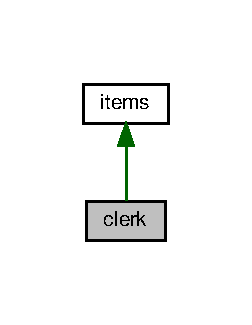
\includegraphics[width=121pt]{classclerk__inherit__graph}
\end{center}
\end{figure}


Collaboration diagram for clerk\+:
\nopagebreak
\begin{figure}[H]
\begin{center}
\leavevmode
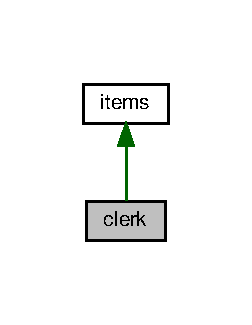
\includegraphics[width=121pt]{classclerk__coll__graph}
\end{center}
\end{figure}
\subsection*{Public Member Functions}
\begin{DoxyCompactItemize}
\item 
\mbox{\Hypertarget{classclerk_aecd9f851adba7385510d8f4fd7186c0c}\label{classclerk_aecd9f851adba7385510d8f4fd7186c0c}} 
char $\ast$ {\bfseries get\+\_\+code} ()
\item 
\mbox{\Hypertarget{classclerk_a1e063c286489b9c7a36c2834095bdc27}\label{classclerk_a1e063c286489b9c7a36c2834095bdc27}} 
float {\bfseries get\+\_\+quantity} ()
\item 
\mbox{\Hypertarget{classclerk_ada10d505eff56232477fb0f8362dac5c}\label{classclerk_ada10d505eff56232477fb0f8362dac5c}} 
void {\bfseries set\+\_\+code} (char code \mbox{[}10\mbox{]})
\item 
\mbox{\Hypertarget{classclerk_aa49972c25b70622815b9a858a4a0a071}\label{classclerk_aa49972c25b70622815b9a858a4a0a071}} 
void {\bfseries set\+\_\+name} (char name \mbox{[}20\mbox{]})
\item 
\mbox{\Hypertarget{classclerk_a58793e4687bda59dd14c06c6543b4985}\label{classclerk_a58793e4687bda59dd14c06c6543b4985}} 
void {\bfseries set\+\_\+price} (float price)
\item 
\mbox{\Hypertarget{classclerk_a0dbebf7f2a33904dd774201e178a288d}\label{classclerk_a0dbebf7f2a33904dd774201e178a288d}} 
void {\bfseries set\+\_\+quantity} (int quantity)
\item 
\mbox{\Hypertarget{classclerk_a94c493b2cb0239a3ebede01f2b6b2f53}\label{classclerk_a94c493b2cb0239a3ebede01f2b6b2f53}} 
void {\bfseries display\+\_\+item} ()
\end{DoxyCompactItemize}
\subsection*{Additional Inherited Members}


The documentation for this class was generated from the following file\+:\begin{DoxyCompactItemize}
\item 
clerk.\+h\end{DoxyCompactItemize}

\hypertarget{classcustomer}{}\section{customer Class Reference}
\label{classcustomer}\index{customer@{customer}}


Inheritance diagram for customer\+:
\nopagebreak
\begin{figure}[H]
\begin{center}
\leavevmode
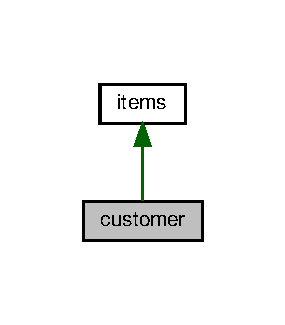
\includegraphics[width=137pt]{classcustomer__inherit__graph}
\end{center}
\end{figure}


Collaboration diagram for customer\+:
\nopagebreak
\begin{figure}[H]
\begin{center}
\leavevmode
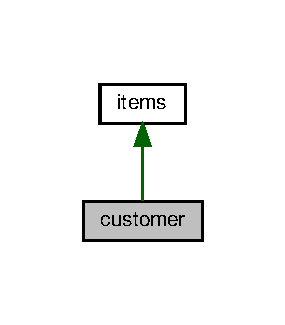
\includegraphics[width=137pt]{classcustomer__coll__graph}
\end{center}
\end{figure}
\subsection*{Public Member Functions}
\begin{DoxyCompactItemize}
\item 
\mbox{\Hypertarget{classcustomer_a1f6e71e10262a93b5bc35bdbad5a6012}\label{classcustomer_a1f6e71e10262a93b5bc35bdbad5a6012}} 
char $\ast$ {\bfseries get\+\_\+code} ()
\item 
\mbox{\Hypertarget{classcustomer_a107b90ba36a4aa9cea24b708cf0718da}\label{classcustomer_a107b90ba36a4aa9cea24b708cf0718da}} 
char $\ast$ {\bfseries get\+\_\+name} ()
\item 
\mbox{\Hypertarget{classcustomer_a5635d635de7211e7a645638b04e9a856}\label{classcustomer_a5635d635de7211e7a645638b04e9a856}} 
float {\bfseries get\+\_\+price} ()
\item 
\mbox{\Hypertarget{classcustomer_a5fd327e9850da893d4d6ddd3382792d3}\label{classcustomer_a5fd327e9850da893d4d6ddd3382792d3}} 
int {\bfseries get\+\_\+quantity} ()
\item 
\mbox{\Hypertarget{classcustomer_a9d9033aea7fa63d5ee43edb6a112cc10}\label{classcustomer_a9d9033aea7fa63d5ee43edb6a112cc10}} 
void {\bfseries set\+\_\+quantity} (int quantity)
\item 
\mbox{\Hypertarget{classcustomer_a5e4916ba70a62e0630471f8a808abe52}\label{classcustomer_a5e4916ba70a62e0630471f8a808abe52}} 
void {\bfseries display\+\_\+catalog} ()
\end{DoxyCompactItemize}
\subsection*{Additional Inherited Members}


The documentation for this class was generated from the following file\+:\begin{DoxyCompactItemize}
\item 
customer.\+h\end{DoxyCompactItemize}

\hypertarget{classitems}{}\section{items Class Reference}
\label{classitems}\index{items@{items}}


Inheritance diagram for items\+:
\nopagebreak
\begin{figure}[H]
\begin{center}
\leavevmode
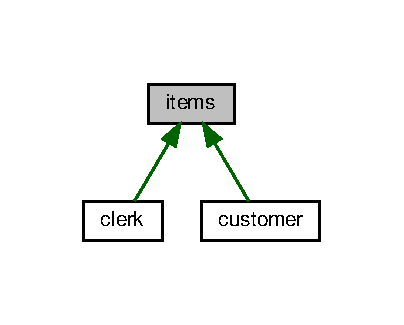
\includegraphics[width=194pt]{classitems__inherit__graph}
\end{center}
\end{figure}
\subsection*{Protected Member Functions}
\begin{DoxyCompactItemize}
\item 
\mbox{\Hypertarget{classitems_a5a7a41e23b095e6096a35454bcb9e6a3}\label{classitems_a5a7a41e23b095e6096a35454bcb9e6a3}} 
char $\ast$ {\bfseries get\+\_\+code} ()
\item 
\mbox{\Hypertarget{classitems_a252aac1b45b345e02bdc2dc867641d1c}\label{classitems_a252aac1b45b345e02bdc2dc867641d1c}} 
char $\ast$ {\bfseries get\+\_\+name} ()
\item 
\mbox{\Hypertarget{classitems_a2dbb4878dd1ea7d30bef82e1c25870b8}\label{classitems_a2dbb4878dd1ea7d30bef82e1c25870b8}} 
float {\bfseries get\+\_\+price} ()
\item 
\mbox{\Hypertarget{classitems_a822e6944c69cff121784f37ae8fc3e53}\label{classitems_a822e6944c69cff121784f37ae8fc3e53}} 
int {\bfseries get\+\_\+quantity} ()
\item 
\mbox{\Hypertarget{classitems_a247847d28799c6f17e3118928c0ea3e1}\label{classitems_a247847d28799c6f17e3118928c0ea3e1}} 
void {\bfseries set\+\_\+code} (char code \mbox{[}10\mbox{]})
\item 
\mbox{\Hypertarget{classitems_a01669ca13ce82885df1579138cfb43a9}\label{classitems_a01669ca13ce82885df1579138cfb43a9}} 
void {\bfseries set\+\_\+name} (char name \mbox{[}20\mbox{]})
\item 
\mbox{\Hypertarget{classitems_aee8fbfc6e786eb09f0817607500c8718}\label{classitems_aee8fbfc6e786eb09f0817607500c8718}} 
void {\bfseries set\+\_\+price} (float price)
\item 
\mbox{\Hypertarget{classitems_a7e750c133d6fe0dac52eb7995f9214ed}\label{classitems_a7e750c133d6fe0dac52eb7995f9214ed}} 
void {\bfseries set\+\_\+quantity} (int quantity)
\end{DoxyCompactItemize}


The documentation for this class was generated from the following file\+:\begin{DoxyCompactItemize}
\item 
data\+Class.\+h\end{DoxyCompactItemize}

%--- End generated contents ---

% Index
\backmatter
\newpage
\phantomsection
\clearemptydoublepage
\addcontentsline{toc}{chapter}{Index}
\printindex

\end{document}
